\documentclass[conference]{IEEEtran}
\IEEEoverridecommandlockouts
% The preceding line is only needed to identify funding in the first footnote. If that is unneeded, please comment it out.
\usepackage{cite}
% \usepackage{hyperref}
\usepackage{amsmath,amssymb,amsfonts}
\usepackage{algorithmic}
\usepackage{graphicx}
\usepackage{textcomp}
\usepackage{xcolor}
\usepackage{url}
\usepackage{flushend}

\def\BibTeX{{\rm B\kern-.05em{\sc i\kern-.025em b}\kern-.08em
    T\kern-.1667em\lower.7ex\hbox{E}\kern-.125emX}}
\begin{document}

\title{Classification of Fanaroff-Riley Radio Galaxies using Conventional Machine Learning Techniques}

\author{\IEEEauthorblockN{Burger Becker}
\IEEEauthorblockA{\textit{Computer Science Department} \\
\textit{Stellenbosch University}\\
Stellenbosch, South Africa \\
17522021@sun.ac.za}
\and
\IEEEauthorblockN{Trienko Grobler}
\IEEEauthorblockA{\textit{Computer Science Department} \\
\textit{Stellenbosch University}\\
Stellenbosch, South Africa \\
tlgrobler@sun.ac.za}
}

\maketitle

\begin{abstract}
Large scale radio astronomy projects such as the Square Kilometre Array (SKA) is expected to produce extremely large data sets (300 PB p/a), which makes purely manual classification no longer a viable option. An automatic method of radio galaxy classification is proposed in this paper that will examine the performance of conventional classification approaches to determine whether accurate classification can be done on subjective features.
This method is meant to act as a tool for domain experts or as an auxiliary function for deep learning classifiers. The morphological features extracted are lobe size, hot spot/peak brightness, the number of lobes present and the Fanaroff-Riley (FR) ratio. To determine the relevance of the morphological features as indicators of class differences, the features are then used in several machine learning classifiers, of which the study compares the classification accuracy and F1-score. Overall, the Random Forest classifier produces the highest accuracy (94.66\%) and F1-score (0.94) using all the features in conjunction. The relevance of the Fanaroff-Riley ratio as a classification metric is verified. Further investigation in automatic extraction of the ratio is required.
% An automatic method of radio galaxy classification is proposed in this paper, which uses a conventional feature extraction based approach combining computer vision techniques and machine learning to differentiate between Fanaroff-Riley type I and II radio galaxies. 

\end{abstract}

\begin{IEEEkeywords}
Machine Learning, Radio Astronomy, Computer Vision 
\end{IEEEkeywords}

\section{Introduction}
The latest radio surveys are expected to provide a deluge of data, for example the Square Kilometer Array (SKA) radio telescope in South Africa is expected to produce nearly 300 PB of data per year \cite{jonas_2018} and the Australian SKA Pathfinder's Evolutionary Map of the Universe has an anticipated output of around $\sim70$ million, sources of which around 7 million might require visual inspection \cite{askap_2008} \cite{emu_2011}. The implication being that  manual classification by experts will no longer be a viable solution \cite{hocking_2015}, although large scale citizen science projects might be a viable alternative.

Methods that provide automated classification is another potential solution, given the recent advances in the field of image recognition and processing. Some examples of automated radio galaxy classifiers that have been developed include: Toothless \cite{aniyan_thorat_2017}, FirstClass \cite{alhassan_2018}, CLARAN \cite{wu_2019} and a comparison between CNN's and Capsule Networks \cite{lukic_2019}, most of which use Convolutional Neural Networks (CNN).

CNN's perform on par with humans at image classification tasks that have a complex feature space, which is difficult to express and model mathematically (such as explicitly modeling the visual differences between a cat and a dog). 


\begin{figure}[h]
    \centering
    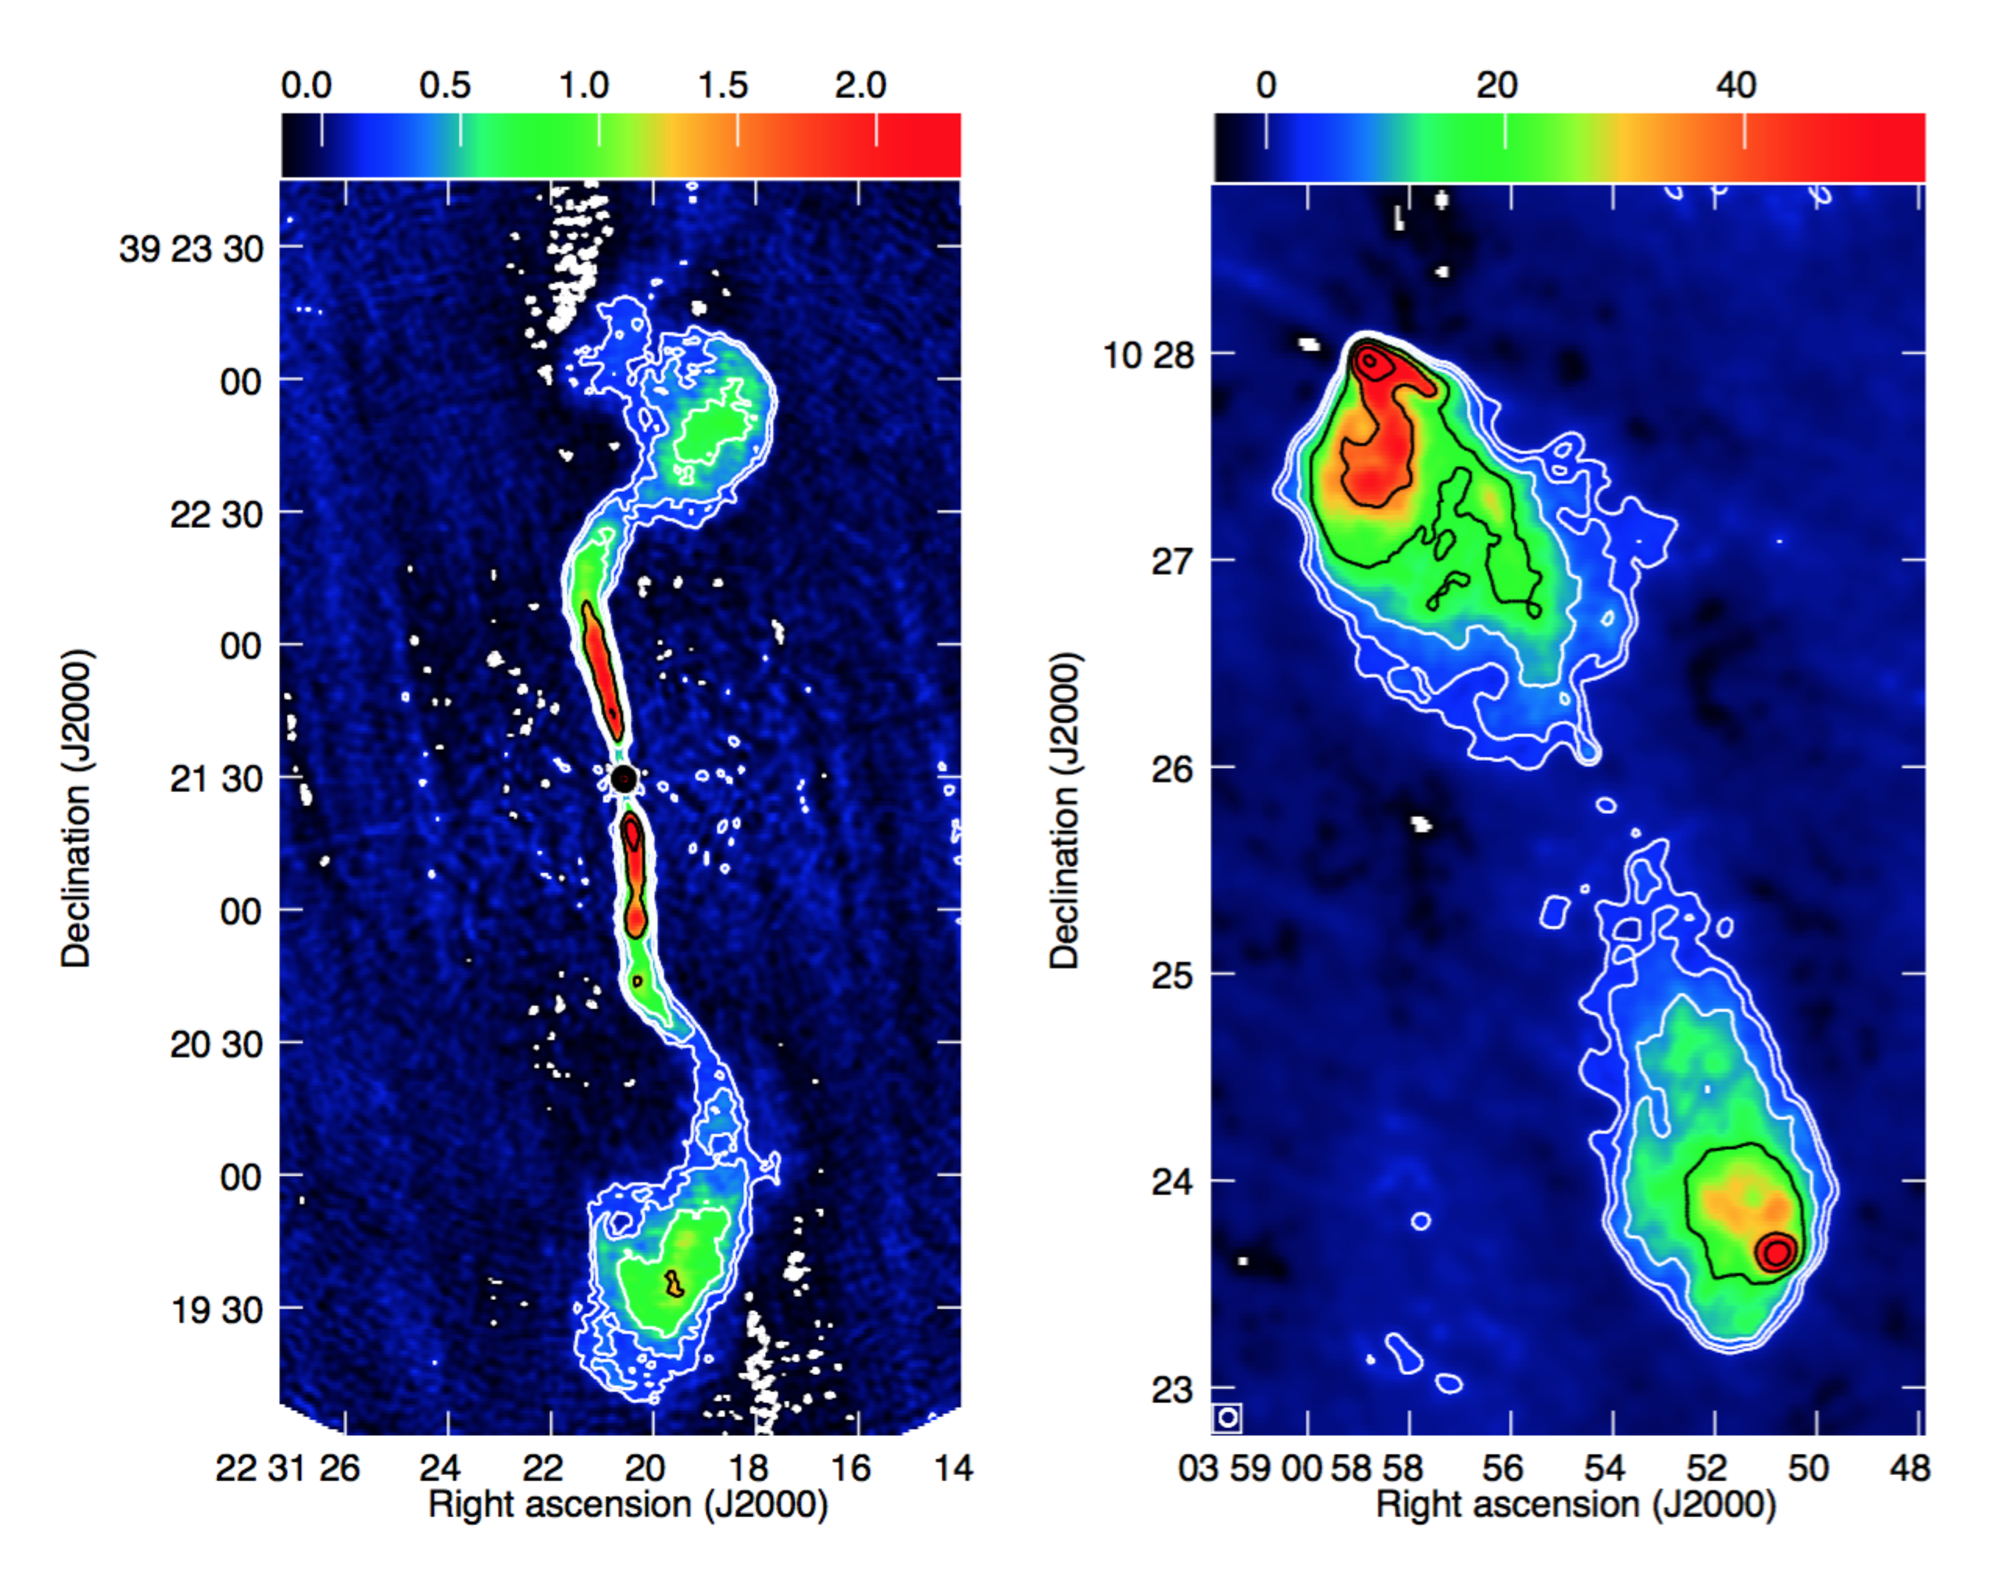
\includegraphics[width=0.5\textwidth]{EPS/kharb2015.eps}
    \caption{The FRI galaxy 3C 449 (left) and the FRII galaxy 3C 98 (right) illustrate the FR morphology. The red area indicates the brightest radio emission. For the FRII's the edges are much brighter in radio emissions, while the FRI's have the hotspots close to the lobes. Reproduced from Extragalactic jets from every angle, Proceedings of the International Astronomical Union, IAU Symposium, Volume 313, pp. 211-218 with permission \cite{kharb2015}}
    \label{fig:kharb}
\end{figure}

A requirement for CNN's is a large amount of training samples, in the range of 10 000 images. Given the relative geometric simplicity of the classification problem and that the current datasets contain in the order of only $\sim1000$ unique sources, CNN's might not be the most appropriate solution. 
Most of the existing systems solve the problem posed by the lack of data by augmenting the existing datasets with rotation and translation of radio sources. This does accentuate the risk of over-fitting by learning features that do not represent general morphological characteristics of a class, but rather that are preeminent within the sample.

A major drawback of CNN's is that we do not know the features being used for classification. There are several methods of analysing these systems, such as filter visualization \cite{aniyan_thorat_2017}. Rather than analysing these systems directly, we propose a method to test if an augmented dataset contains potential subjectivity. An ``objective'' feature can be described as a characteristic of the data that is a consistent quantifiable metric which is independent of other factors. For example, the radio telescopes's resolution has an effect on the area in the visual representation of the source. Area in this case is quantifiable in pixels but radio telescope's with different resolutions will result in an inconsistent value. This is expanded on in the results section.

The Fanaroff-Riley (FR) classification scheme provides an objective feature in the form of the FR-ratio \cite{fanaroff_riley_1974}. Within this scheme, extra-galactic radio sources were originally divided into two classes, namely FR type I and type II. Type I and type II sources are describes as being edge brightened and lobe brightened, respectively. Because the ratio is not dependent on external features and is a self-contained metric, it acts as an example of an objective feature.

In contrast to CNN's, most conventional Machine Learning methods require relatively few samples (such as Random Forest), compared to Deep Learning and have not been examined in much depth for radio source classification. This paper will examine the performance of conventional classification systems to determine whether accurate classification can be done on subjective features.

In practice, the FR-ratio is but one of a host of features being used during manual classification by experts. Within the literature there is no 
clearly defined set of visual features for FR classification. Rather it seems that
becoming proficient at classification is more dependant on a mix between domain 
specific knowledge, experience classifying the data and an intuitive grasp of the class differences. 

The focus of this paper is to examine the role the FR ratio plays in 
classification, to clarify the additional morphological features which are subjective or objective, and to attempt to set up classifiers based on those features examined. 
These tools can then be used in tandem with the experts to ease and speed up classification.

In summary, we will investigate:

\begin{itemize}
\item if conventional Machine Learning morphological features can be used to classify radio galaxies
\item present an approach which can detect if small radio galaxy datasets contain subjective morphological features that add to class seperability. This may lead to the CNN being biased in a specific way by the subjectivity inherent in the dataset.
\item examine whether the FR-ratio is still a relevant feature for radio galaxy classification 
\end{itemize}



\section{Literature Review}

\subsection{Radio Astronomy Background}

Radio galaxies are active galaxies that are strong emitters of
radio waves powered by accretion onto a super massive black hole that produce extended structures called radio jets and lobes \cite{wierzbowska_2011}. The FR-ratio is defined as the distance between the regions of highest brightness (hotspots) on opposite sides of the active galactic nucleus (AGN) and the distance between the farthest edges of the lobes. Sources where the ratio is less than 0.5, are classified as FRI and all sources greater than 0.5 is placed in FRII (fig.\ref{fig:becker2019}). 
\begin{figure}[h]
    \centering
    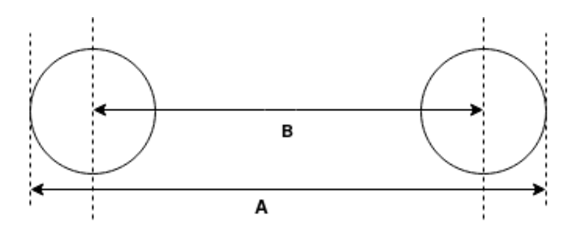
\includegraphics[width=0.5\textwidth]{EPS/ratio_becker.eps}
    \caption{A diagram of the Fanaroff-Riley ratio. The ratio is defined as the inter-lobe hotspot distance (B) divided by the total source length (A)}
    \label{fig:becker2019}
\end{figure}
% Another, more concrete definition that has been given is by Owen and Ledlow \cite{owen_1994} based upon the relationship between optical luminosity and radio luminosity. Examining a classification system based on optical features is outside of the scope of this project and would require optical catalogues being correlated with radio catalogues.



% \begin{figure}[h]
%     \centering
%     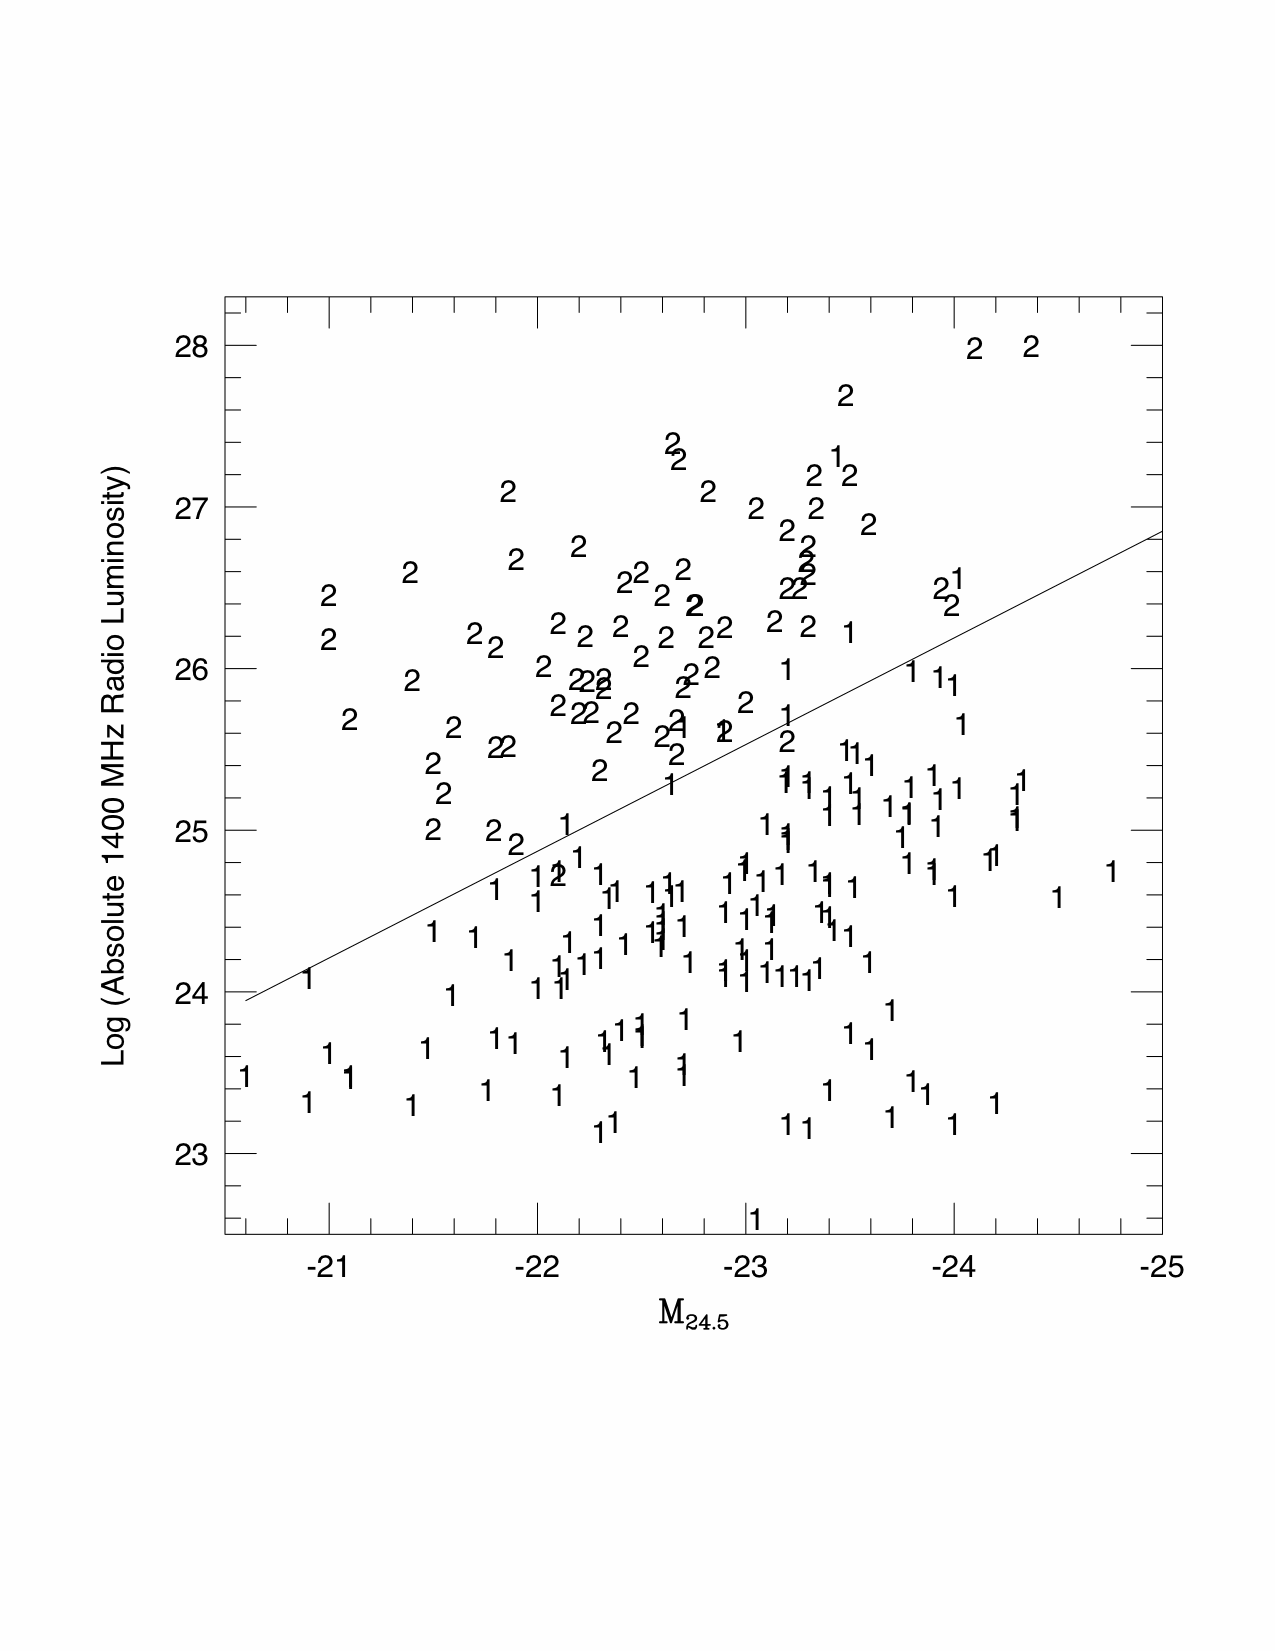
\includegraphics[width=0.5\textwidth]{Owen_ledlow94.png}
%     \caption{FRI as 1 and FRII as 2 (Owen \& Ledlow, 1994)}
%     \label{fig:owen1994}
% \end{figure}



Alternative classification schemes have been proposed with the ratio at 0.8, based on catalogues with better resolution than the Third Cambridge Catalogue of Radio Sources that was used by Fanaroff and Riley. 
The study by Lin et al. \cite{lin_2010} proposed a ratio $r = S/T$, with $T$ being the total length of the radio source and $S$ being the distance between highest surface brightness spots on either side of the AGN. The conclusion of that study was that such a ratio had limited application in classification of radio galaxies, due to overlap in physical properties of the two different groups that leads to a smooth transition between FRI and FRII classes rather than a sharp class distinction. This study used no other morphological features for classification.
% All the ratios calculated in these studies have been done by hand, but no large scale computer vision and machine learning study has been performed that rigorously and statistically verifies the accuracy of the ratio as a useful morphological feature. Lin et al. \cite{lin_2010} also proposes ``to define an 
% objective measure (or measures) that allows us to trace the galaxy population 
% smoothly from FR type-I-like sources to type-II-like ones (as opposed to a sharp 
% and perhaps arbitrary type I versus type II division). With the aid of such a 
% measure, we hope to reduce the subjectiveness inherited in the traditional ways of
% classification, thus increasing the repeatability of our results by other 
% researchers''.

% While their study has provided ground work for such a scheme and laid out several measures to perform classification, no uniform tool-set has been developed for this
% purpose and their own methodology has similar issues to previous schemas: a lack of an objective measure and subjective qualities inherited due to the lack of well defined features that they were using during morphological classification or rigorously defining their algorithm for repeatability and verification of results.
Other sources in the literature provide other potential morphological features, 
such as the presence of jets \cite{owen_laing_1989} or hotspots towards the edges of 
the lobes \cite{gendre_wall_2009} as well as the number of hotspots present \cite{lukic2018}.

\subsection{New Classes: Beyond FRI and FRII}
% The main problem with classification is that the possibility remains that your data isn't separable by the features you have chosen or new more detailed data starts to blur the class lines.
Since the FR-ratio's inception, several new classes have been proposed as higher resolution catalogues have been made, such as Bent tails. Bent tails are further subdivided into Wide Angle Tails and Narrow Angle Tails. In addition to these, there are sources that seem to have hybrid morphologies, known as HyMORS \cite{gopalkrishna2000} that display qualities of an FRI in one lobe and FRII in the other. These additional classes are outside the scope of this paper, but is important to understand the complexity of the classification landscape.

% \subsection{Radio Galaxy Catalogues}
% Different definitions of FRI/FRII's have developed in the academic community. 
% % Initially, I used the FIRST catalogue and FRICAT. However, the problem with these catalogues are that they contain compact sources within them, which completely throw off any hopes of a ratio based classification method. Compact sources are defined as unresolved sources having a single non-diffuse hot-spot \cite{lukic2018}. Part of the catalogues we currently use for FRI and FRII are FRICAT (Capetti et al. 2016) and FRIICAT (Capetti et al. 2017) , respectively. Both of these were composed from several other catalogues: NRAO VLA Sky Survey (NVSS) (Condon et al. 1998), Faint Images of the Radio Sky at Twenty Centimeters (FIRST) (Becker et al. 1995) and the Sloan Digital Survey (SDSS) (York et al. 2000).
% FRICAT consists of 219 FRI galaxies and FRIICAT of 122 FRII galaxies. Each of the three authors of FRIICAT performed manual inspection for each source independently, after which they only included sources where at least two of them agreed that it was a FRII.

\subsection{Machine Learning}
A meta-study done by Feigelson \cite{feigelson} with regards to classification 
methods used in astronomy found that the majority of studies used neural networks
($\sim150$ studies, 1990-2006), commenting that although this method is quite effective, 
it gives ``black box'' results: difficult to reproduce and very little insight into 
the feature space used. The majority of classifiers set up between then and now 
have been neural networks, albeit these were the more recently developed 
Convolutional Neural Networks (CNN) \cite{hinton_2012}. An example classifier is Toothless \footnote{\url{https://github.com/ArunAniyan/RadioGalaxyClassification}}  \cite{aniyan_thorat_2017}, with which we shall be comparing our results later on. Very few studies used 
Bayesian classifiers (~30 studies, 1985-2006) or decision trees (~20 studies, 
1994-2006) and none used Classification and Regression Trees. Note that not all of these classifiers were set up for radio astronomy, as some of these studies focused on optical astronomy.





% \subsection{Deep Learning}
% There has been significant work done on creating Deep Learning classifiers in radio astronomy as was mentioned in the introduction, such as the Radio Galaxy Zoo project's \cite{lukic2018}
% Looking at existing CNN's trained for classification \cite{lukic2018} and 
% identifying the features that it is looking at will be of extreme importance. This 
% can be done by methods such as image retrieval by scene graph grounding (Johnson et 
% al. 2015) and visualizing of the CNN (Zeiler \& Fergus, 2014) to name a few 
% methods.
% The importance of feature selection is much clearer in a case such as 
% this. Classification without explanation or feature models to back it up leaves 
% astronomy (or in the general case the field we're applying these methods to) in a 
% precarious position: classification might no longer coincide with actual physical 
% characteristics of radio galaxies (or what the relevant subject matter may be).
% potentially undoing research from data labeled by automatic classifiers that have not undergone rigorous feature selection andengineering. 



\section{Methodology}
The order of implementation was image preprocessing, manual calculation of the ratio, automatic ratio and feature extraction and then setting up classifiers given those features.

\subsection{Dataset Description}
The sample selection for this study is based on the one used by Aniyan and Thorat from the Toothless classifier \cite{aniyan_thorat_2017}, with the exclusion of the Bent-tailed radio sources in their sample selection. This includes 219 FRI sources from FRICAT \cite{capetti_2016}, 71 FRI's and 464 FRII's from CoNFIG \cite{gendre_wall_2009}.
% By visual inspection, we have found several compact sources and sources which would be classified as Bent tails. This can possibly have an influence on the quality of the model.
\subsection{Image Processing}
There is a high level of noise in most of the images that provides a significant hurdle for automatic classification methods, especially identifying separable lobes within the actual galaxy body. There are two parallel processing steps that are used in conjunction and this is shown in fig. \ref{fig:imagepipeline}. The first step taken is a binary threshold of the image using sigma clipping that returns a threshold of of everything above one standard deviation of the image. This covers the main body that we are interested in but still includes residual smaller bodies that are not useful. The image is labeled after thresholding by using the Scipy Label package \cite{scipy}. In order to further isolate only those bodies we are interested in, Singular Value Decomposition (SVD) is used to reconstruct the image using only the Principle Components that account for 90\% of the variance of the image. A binary threshold is then applied to this SVD reconstruction, which is then used in conjunction with the former clipped image threshold to create an image of the lobes from the original image that had been kept in the SVD reconstruction. The preprocessing method still requires statistical verification in order to assert that the technique generalises well on larger datasets. 
% The pipeline is laid out in figure \ref{fig:imagepipeline}.

\begin{figure*}[h]
    \centering
    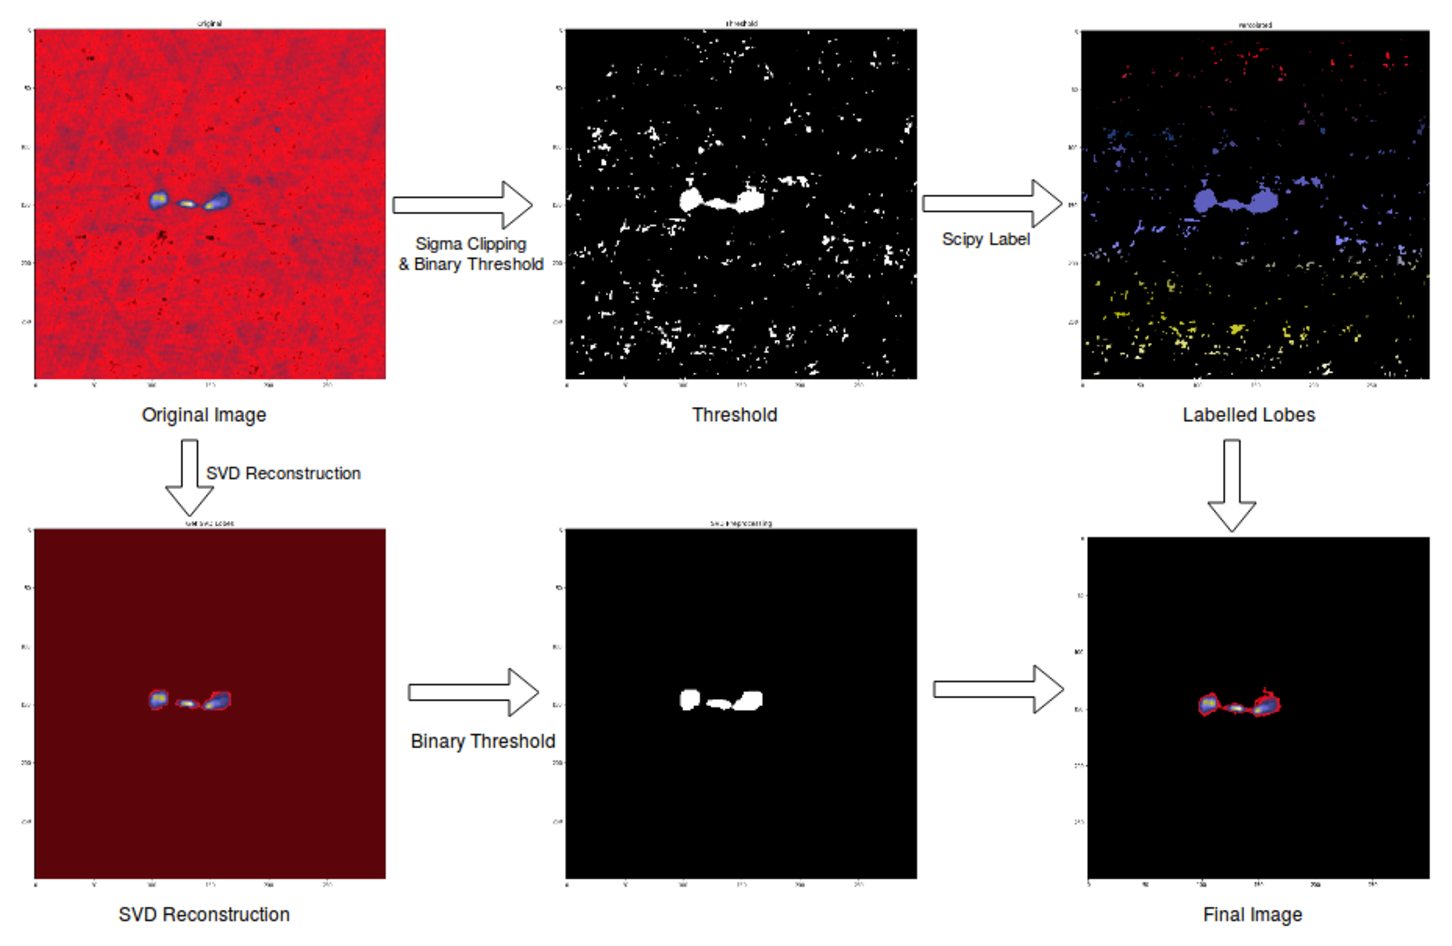
\includegraphics[scale=0.5]{EPS/pipelines.eps}
    \caption{Image Preprocessing Pipeline}
    \label{fig:imagepipeline}
\end{figure*}

\subsection{Image Segmentation}
According to Fanaroff and Riley's original paper on the matter, the ratio can be calculated by taking the distance between the two brightest areas on the lobes, either side of the AGN, and dividing that by the total distance between the furthest contour of the edges on either side (i.e. more or less in line with the line between the brightest hotspots).

Machine learning is useful in the preprocessing of the data as well, especially when certain semantic distinctions are needed to be made without much prior knowledge of these class distinctions. In order to determine the relative positions of hotspots to the lobe edges, an unsupervised method is required to cluster the image into three main semantic categories: background, lobes and hotspots. The need for an unsupervised algorithm arises from the differences in radio luminosity between classes and within classes if sources are from different catalogues.
% The main issue arising with this is separating the background and the source in question.
% Segmentation is one way of isolating the parts of the image that we are interested in. 
Well established machine learning methods such as the k-means 
algorithm \cite{macqueen1967} can be useful ways to 
cluster these pixels into the three categories we have discussed and to start the automatic feature extraction process. We have made use of the Scikit-Learn implementation of k-means \cite{scikit-learn}. 
% The k-means algorithm can be made more efficient by choosing the initial cluster positions intelligently (Bradley et al. 1998).

The technique we developed for manual classification involves visually inspecting the image under at least two different colour maps, inspecting its k-means segmented version, starting at 3 clusters and then increasing the number of clusters if higher levels of detail is required. Finally, a method of blocking out the 10 brightest pixels at a time was used. Once there is a blocked out pixel that is separate from the rest, one can safely assume that you have found a hotspot (best method). This method does make some assumptions, such as that the AGN lobe will always be the brightest and not one of the side lobes.

\subsection{Manual Ratio Extraction Tool}

In order to manually calculate the FR-ratio, we set up a software tool to aid us in classification. The tool's functionality include various methods of visualising the images\footnote{\url{https://github.com/BurgerBecker/radio-galaxy-conventional-classifier}}. This is done through using different colour maps  and other methods such as K-means clustering, which clusters different pixels together into k number of clusters. 
Setting k to 3, what we attempt to find is whether the distinction between background, lobe and hotspot pixels can be made through this grouping. This leads to the interesting question of what k should be and whether those values should then be further compressed down to the 3 classes we want.

The tool can then be used to calculate the ratio by clicking upon the points you want to designate as hotspots and the furthest edge points from both these hotspots. Note that these points are subject to the manual classifier's interpretation of where this point should be and how in line these edge points are with the hotspots.

\subsection{Manual Calculation of FR-Ratio}
Manual ratio calculation was a necessary component in order to set a baseline for automatic ratio calculation. We calculated the ratios of a large portion of the data-set and calculated the ratio for 72 FRI and 78 FRII images.

This exercise was also meant to provide better first hand understanding of the subject matter and to see how a human would learn to classify radio galaxies themselves (the reason for which is expanded upon more within future work). This also  gave rise to the understanding why this calculation is difficult to formalize into an algorithm (due to the sometimes objective nature of what a hot-spot is relative to the other points). Potential improvement on this can include two or three subject matter experts calculating the ratio and cross referencing these for errors.

\subsection{Automatic Ratio Extraction}
After the image has been preprocessed, the necessary features can be extracted for the FR-ratio's calculation. This involves finding the AGN, hot-spots either side of the AGN and calculating the distances from each of these to the furthest contour edge of the source. The AGN is found by calculating the centre of mass of all the lobes within the body and taking the lobe closest to that one as the AGN. The line of best fit is then calculated between the hot-spots of the different lobes, in order to determine the line of symmetry. This could be useful in the future to homogenize other datasets by removing rotation as a factor. The brightest hot-spot either side of the AGN is then taken. This method does not generalise well on the dataset, due to low lobe and hotspot separability in FRI's from the AGN, which make it hard to identify where a hotspot begins (as can be seen in fig. \ref{fig:kharb}).

\begin{figure}[!h]
    \centering
    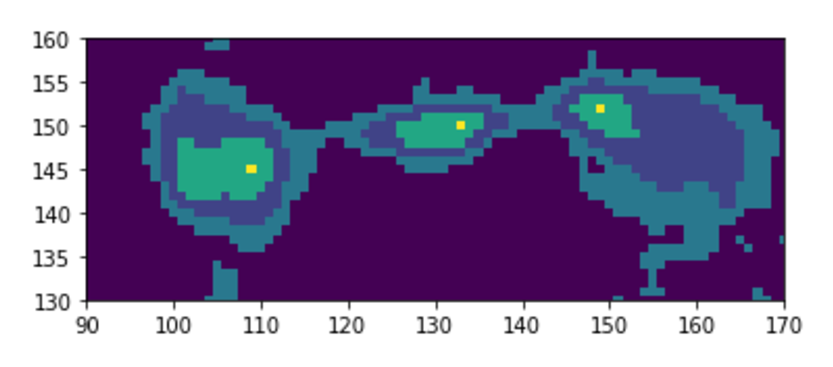
\includegraphics[width=0.5 \textwidth]{EPS/hotspots.eps}
    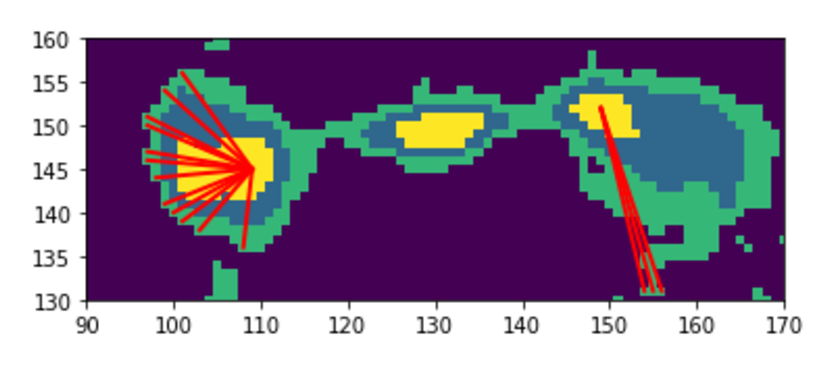
\includegraphics[width=0.5 \textwidth]{EPS/findingfurthestpoint.eps}
    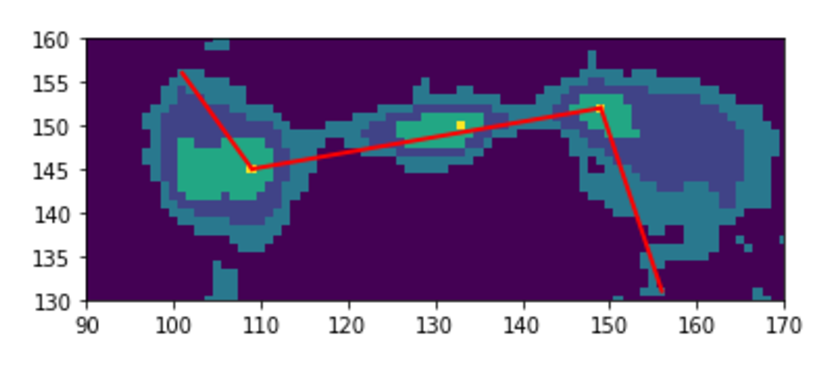
\includegraphics[width=0.5 \textwidth]{EPS/ratioauto.eps}
    
    \caption{Automatic hotspot detection: 1. Finding the hotspots, 2. Finding the furthest contour edges, 3. The calculated ratio}
    \label{fig:hotspotsss}
\end{figure}

\subsection{Feature Description}

As a proof of concept, a relatively simplistic classifier has been set up in order to see whether there is class separability among the features we have selected to extract. 

A brief description of the four features we initially extracted. The first is the total lobe area in the image after preprocessing. This is simply a sum of the pixels after a binary threshold has been applied. Establishing whether this is a good or bad feature on our dataset is important, for in theory absolute area should not be a deciding feature. Both FRI's and FRII's can possibly be at any distance from Earth, which at a given resolution will result in a different size for the same class of object. If this area feature on its own acts as a good feature, we should be aware that the dataset does not include the scale variance that real world data can possibly have.

Number of separable lobes present within the central body is our second feature. A single lobe is defined as a group of neighbouring pixels that have a non-zero value after preprocessing. By the definition of FRII's being edge brightended and FRI's being lobe brightened, we can expect denser core regions for FRI's and less separation between the lobes.

Hotspot brightness was picked as an important feature due to it being one of the defining characteristics of the FR dichotomy.

Both brightness and area are subjective features in this case, due to the area being dependant on the resolution of the telescope making the observation.

Automatic feature extraction was performed on a dataset of 290 FRI's and 464 FRII's.

\subsection{Feature Extraction}

The features that were automatically extracted include the total area of all lobes kept after preprocessing (referred to as Area from here on), the intensity of the brightest hotspot in the image (referred to as hotspot or HS in all relevant tables) and the number of distinct lobes present in the image after preprocessing (referred to as Number of Lobes or NL in all relevant tables).

Additional features that can be used is AGN lobe size relative to total area (which would be a more scale invariant feature than merely area size, that should theoretically not be a good feature due to the radio source not being on similar distances from Earth), intensity of the brightest hotspot in other lobes.

\section{Experiments and Results}

This section gives the results from two experiments: $A-D$ the data with a manually calculated ratio (with Ratio as a Feature) and $E-F$ the full dataset with no ratio component (Automatically Extracted Features).

\subsection{Baseline Classifier on Raw Images}

For a baseline classification result, a Gaussian Naive Bayes classifier was set up using the Scikit-Learn package in Python \cite{scikit-learn}. This classifier was fed the raw image data before and after preprocessing. Raw image classification gave a test accuracy of 51.6\% and an F1 score of 0.49 while preprocessing increased test accuracy to 65\% and the F1 score to 0.53. 
% This indicates that preprocessing does keep features that make classification easier among class lines.

\subsection{Classifier Testing with Ratio as a Feature}

Classifier comparison was done using the following in-built Scikit-Learn classifiers: Nearest Neighbors, Linear Support Vector Machine (SVM), Radial Basis Function SVM, Gaussian Process Regression, Random Forest, Multi-layered Perceptron Neural Network, AdaBoosted Decision Tree, Naive Bayes and Quadratic Discriminant Analysis. These classifiers were tested on a combination of the extracted features: Area, Number of Lobes, Brightest Hotspot in the image and the manually calculated ratio. This was done only with a single train-test split at a 33\% test set size, the results of which are in table \ref{tab:freq}. Overall, Random Forest gave the best results on this data. Including the ratio has an increased effect on overall accuracy.

\begin{table*}[h]
  \caption{Table of Most Accurate Classifiers by Features Used}
  \label{tab:freq}
\begin{center}
\begin{tabular}{|c|l|c|l|c|}
    \hline
        Features used & Test Accuracy (\%) & Classifier & F1 Score & Classifier \\
        \hline
        \textbf{Area, HS, NL, Ratio} & \textbf{94.66} & \textbf{Random Forest} & \textbf{0.94} & \textbf{Random Forest}\\
        \hline
        Area, HS, NL & 90.66 & Random Forest & 0.88 & Random Forest \\
        \hline
        Ratio, HS, NL & 90.66 & Nearest Neighbors & 0.89 & Decision Tree \\
        \hline
        Ratio, HS & 92 & Nearest Neighbors & 0.90 & Nearest Neighbors \\
        \hline
        Ratio, NL & 78 & QDA & 0.73 & Neural Net  \\
        \hline
        Area, NL & 77.33 & Linear SVM & 0.7 & Linear SVM \\
    \hline
\end{tabular}
\end{center}
\end{table*}

\subsection{Evaluating the Ratio as a Feature}

In figure \ref{fig:pairwise}, we compare the four selected features in a pairwise plot with a kernel density estimation plot for the two features per class on the main diagonal. There is significant overlap between the features (Lin et al. \cite{lin_2010} noted this in their study on the ratio), however there are clear correlations between specific classes and features, such as the majority of FRII's having a smaller area while the FRI's are more spread out. The ratio's plot in \ref{fig:ratio_plot} shows that while there is class separability using the ratio, a class division boundary is slightly lower than 0.5. 

\subsection{Best Performing Classifier Setup}

The random forest classifier was set up with a maximum tree depth of 5, the number of estimators 10 (also seen as the number of trees in the forest) and the number of features to consider when looking for the best split as 2.

\begin{figure}[ht]
    \centering
    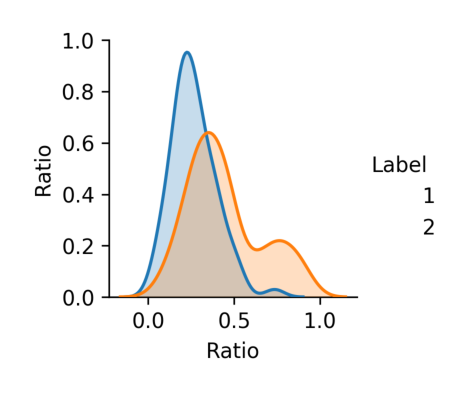
\includegraphics[width=0.3 \textwidth]{EPS/ratio.eps}
    \caption{Manual ratio calculation}
    \label{fig:ratio_plot}
\end{figure}

After using cross validation with a K-fold value of 5, this resulted in a mean accuracy of 0.91 (+/- 0.05). Increasing the maximum tree depth to 15, the number of trees 300 and the number of features at 2 results in an accuracy of 0.89 (+/- 0.02).

\begin{figure}[ht]
    \centering
    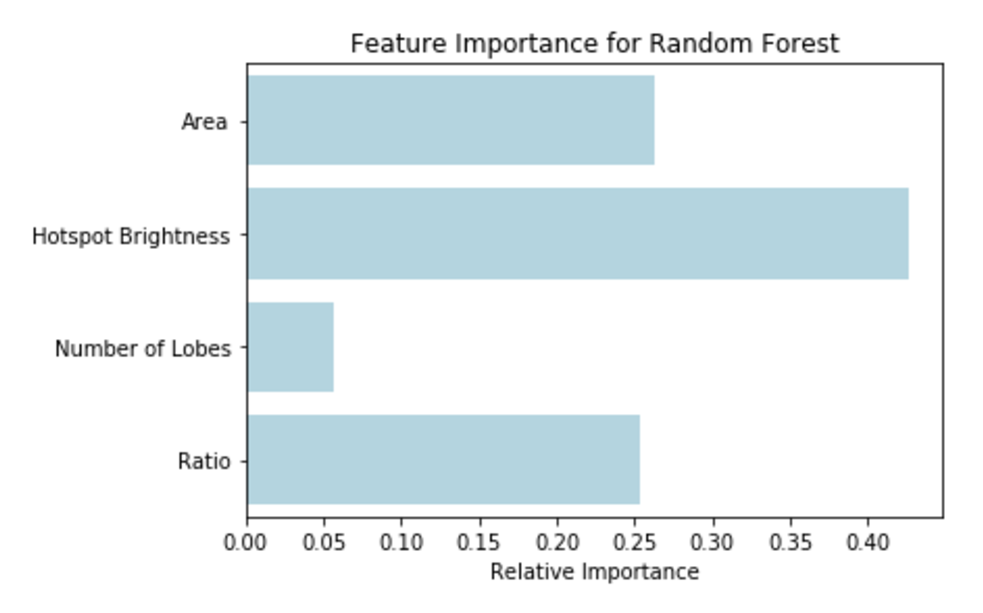
\includegraphics[width=0.5 \textwidth]{EPS/feature_import.eps}
    \caption{Variable importance as given by Random Forest GINI index on the Manual Ratio Extraction Dataset}
    \label{fig:gini}
\end{figure}

\begin{figure}[ht]
    \centering
    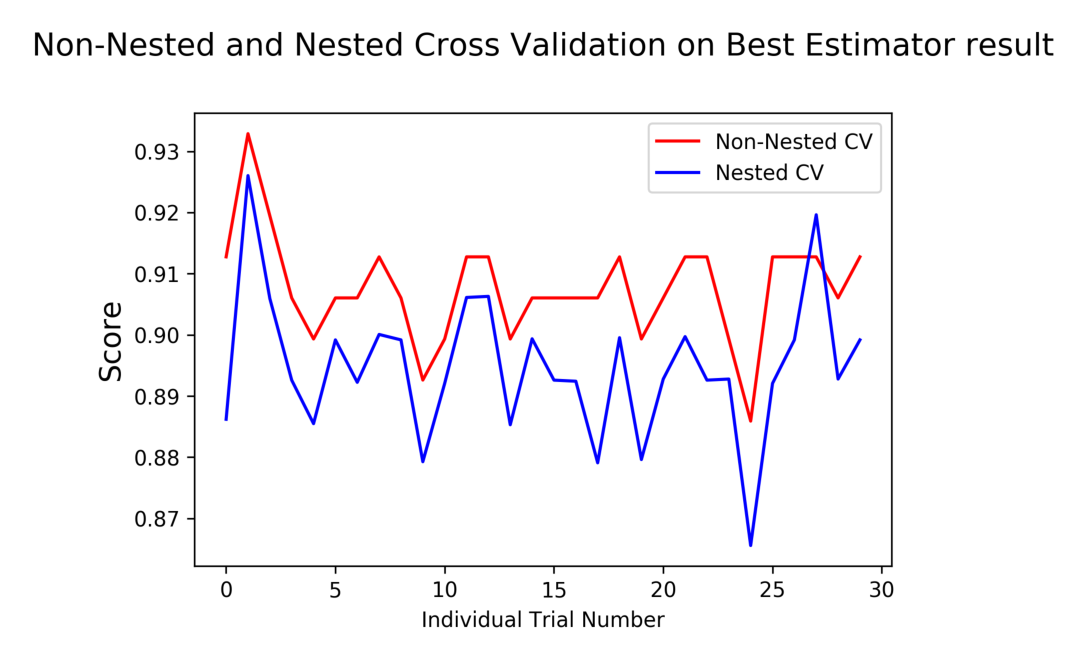
\includegraphics[width=0.5 \textwidth]{EPS/ee.eps}
    \caption{Non-nested cross validation vs Nested cross validation on the Best Estimator Result on the Manual Ratio Extraction Dataset}
    \label{fig:nested}
\end{figure}

We then preform a Grid search using \texttt{Sci-kit Learn's} Gridsearch package that resulted in an optimized random forest classifier with a maximum depth of 10, number of features at 1 and the number of estimators at 500. Then we compare this classifier's accuracy on nested and non-nested cross validation, with non-nested cross validation resulting in an accuracy of 0.91 (+/- 0.02) and the nested cross validation resulting in an accuracy of 0.89 (+/- 0.02). This is illustrated in figure \ref{fig:nested}.

\subsection{Automatic Extracted Feature Results}

Building on this, we seek to find a classifier that generalises on features we can extract with certainty. Initial attempts at automating ratio extraction had failed on roughly 40\% of the data and was left out of this section. In addition to the first four features discussed, two additional subjective features were added to this case: active galactic nucleus (AGN) area and AGN hotspot brightness. We perform a grid search in conjunction with nested cross validation to train a Random Forest classifier. The Random Forest classifier with a maximum depth of 5, number of estimators at 300 and the number of features at 1.

The feature importance is given by figure \ref{fig:agnfeat}, which differs significantly from figure \ref{fig:gini}, with much less importance placed on any single feature. In fact, our most significant feature previously (Hotspot Brightness) has dropped in feature importance to third place, while area and AGN area seem to play a much bigger role. Number of lobes, which is technically our only objective feature, now has a much larger role as well. There are some cases where the number of lobes is calculated much higher than is expected (some cases giving above 10 lobes). This is due to some sources having high levels of noise and a lack of large distinguishing bodies. 
% SVD preprocessing works the best when there are large continuous lobes.

The average accuracy of this last classifier is: 0.9191 (+/- 0.000034).

\begin{figure}[h]
    \centering
    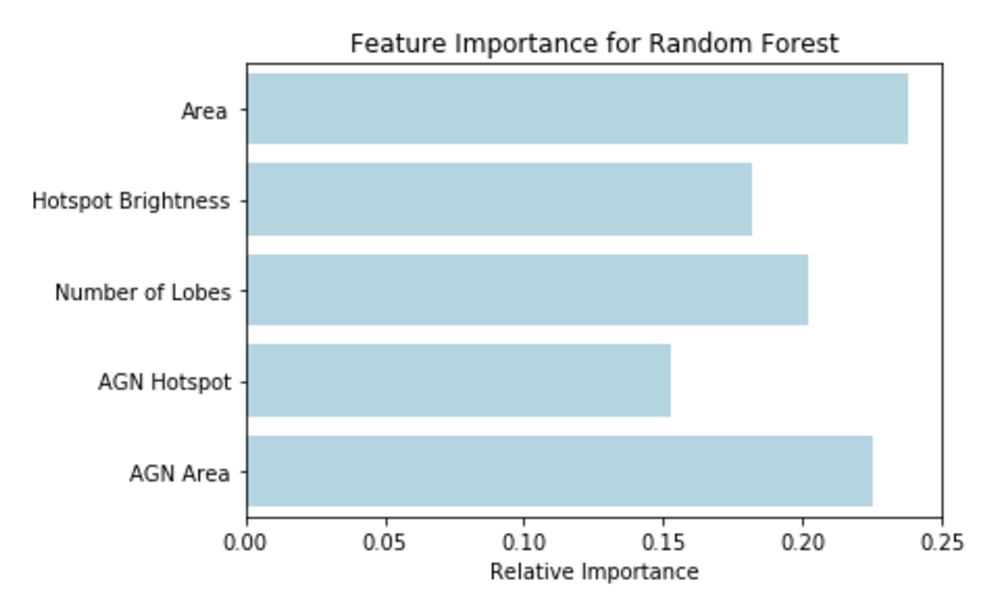
\includegraphics[width=0.5 \textwidth]{EPS/agnfeat.eps}
    \caption{Variable importance as given by Random Forest GINI index on the fully Automatic Extracted Dataset}
    \label{fig:agnfeat}
\end{figure}
\begin{figure}[h]
    \centering
    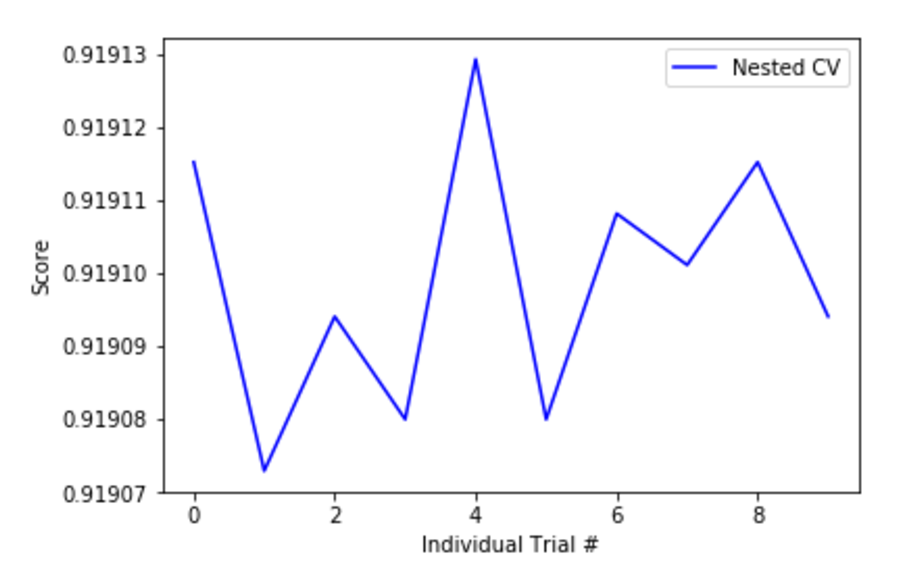
\includegraphics[width=0.5 \textwidth]{EPS/nestedlast.eps}
    \caption{Nested cross validation on the Best Estimator Result on the fully Automatic Extracted Dataset}
    \label{fig:nested2}
\end{figure}

\begin{figure*}
    \centering
    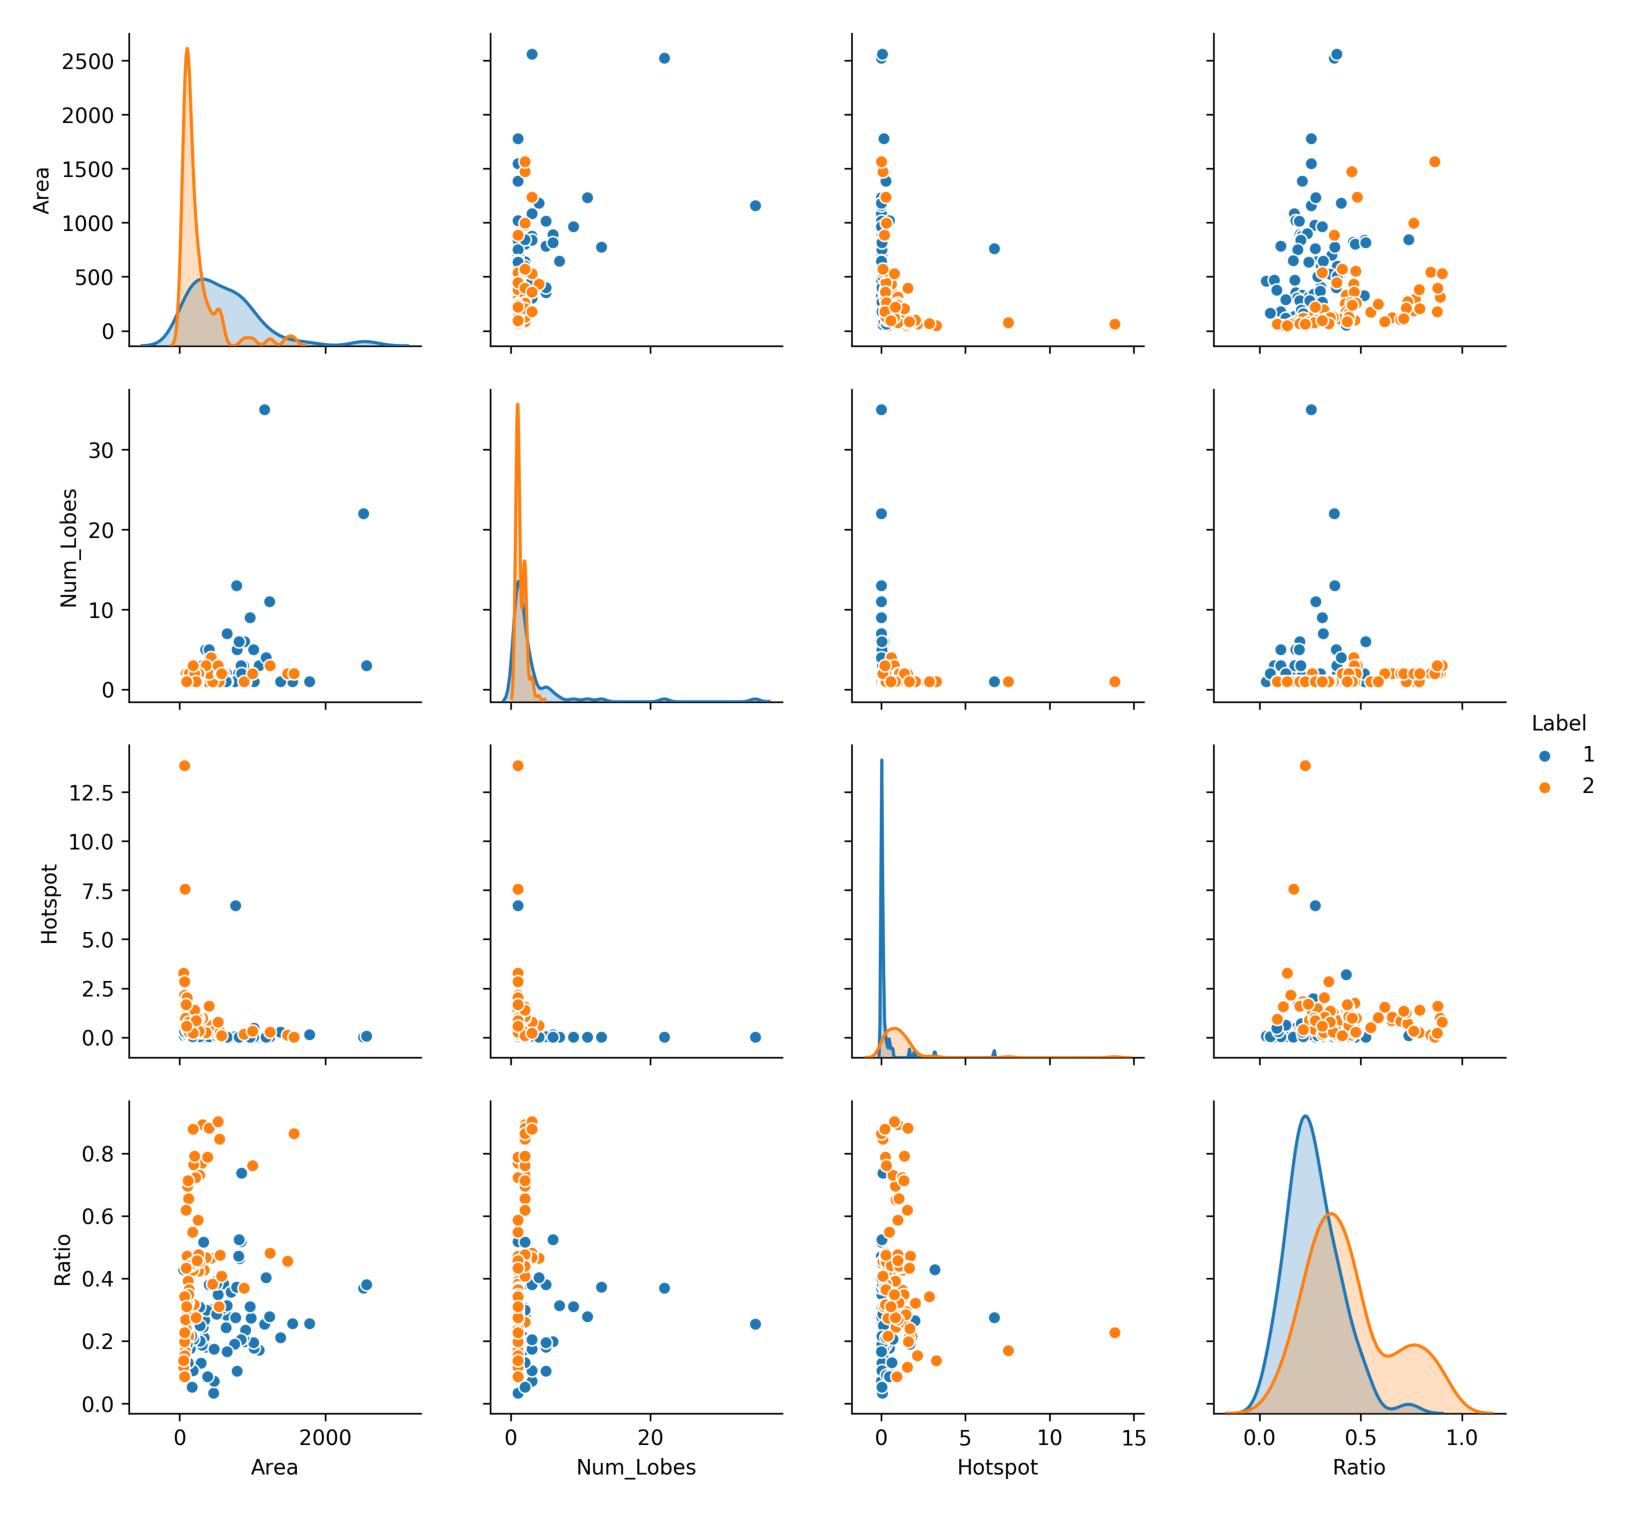
\includegraphics[width=\textwidth]{EPS/pairwise.eps}
    \caption{A pairwise plot of the four features in conjunction with manual ratio that have been selected}
    \label{fig:pairwise}
\end{figure*}

\subsection{Comparison with Deep Learning}

We compare the results of our final classifier with the results of Aniyan and Thorat on Toothless \cite{aniyan_thorat_2017}. Our comparison is limited to this classifier because it was trained and tested on the same dataset. Our results are shown in table \ref{tab:results}.

\begin{table}[h]
  \caption{Result comparison with CNN trained on the same data}
  \label{tab:results}
  
\begin{tabular}{|l|l|l|l|l|}
\hline
Paper & Class & Precision (\%) & Recall (\%) & F1-Score (\%)  \\
 \hline
Aniyan \cite{aniyan_thorat_2017} & FRI & 91 & 91 & 91  \\
 \hline
Aniyan \cite{aniyan_thorat_2017} & FRII & 75 & 91 & 83   \\
 \hline
Own Results & FRI & 100 & 78 & 88 \\
 \hline
Own Results & FRII & 88 & 100 & 93 \\
 \hline
\end{tabular}
\end{table}

\section{Conclusion}

Our main conclusion from the above results is that the Fanaroff-Riley ratio can still be a useful feature to use when classifying radio galaxies. However, from the manual extracted data it is not certain that the optimal ratio split is at 0.5. Classifying based on the manually extracted ratio, we find a more accurate ratio split at a value slightly lower than 0.5.

The ratio in itself is not a class distinguishing feature on its own and should not be used as a the only classification metric. It is, however, a useful objective feature to be used in conjunction with other extracted morphological data. This can be seen from fig. \ref{fig:gini} where the Random Forest's GINI index gives the relative feature importance's, where it is weighted to around 25\% of influence to classification relative to the other features.

Hotspot brightness and lobe area are the two features that contribute the most in fig. \ref{fig:gini}, but are subjective features that do not directly relate to objective measurements in a consistent manner. Both are dependant on the radio telescope's resolution and should be used as features or comparison metrics only if this is taken into account. These subjective features can easily become the dominant features in small datasets such as ours. The possibility exists that the features that deep learning models learn are subjective features, which might not translate well to sources found by the next generation of radio surveys.

The results from our conventional classifier is comparable to the results from convolutional neural networks and shows that there is significant room to make use of conventional feature engineering based approaches towards radio galaxy classification. 
% The computational resources required for this would be significantly lower than what is required for a comparable CNN, in terms of training the model and setting up a running version.

% Since we expect a massive influx of data, we need to consider the time it would take to retrain the model. 

In conclusion, a conventional machine learning approach has merit for a problem such as this one, which might be labeled as a medium complexity issue in morphological classification, due to the lack of highly complex visual features (such as the case in scene identification or animal classification). 
% Using methods such as a CNN for a case where the feature space is already well mapped out is a grievous misuse of computational resources for where conventional methods can deliver similar and even slightly better results. 

The benefits of the conventional approach is shorter training time, with less risk of overfitting the model, shorter time requirement to retrain on new data and more knowledge of feature importance during classification.

The limitations of this model is that the features have to be modeled and extracted.

\section{Future Work}

Converting some of the subjective features to objective features is work that should be examined in more depth, such as extracting the ratio of the source area to a bounding box around it. Calculating the flux density of a source and then comparing this with optical luminosity might be one way to make the brightness an objective measure.
% , which could build on the classification system proposed by Owen and Ledlow \cite{owen_1994}.

A speed and computational resource use comparison between the conventional and deep learning classifiers is necessary in order to evaluate the cost effectiveness of using these classifiers in practise. Evaluating their performance and assessing the need for specialised hardware is important for large scale projects such as the SKA.

% Future work on this project would include setting up a deep learning model with augmentation techniques (scaling and rotation) that are different than the ones used by Aniyan and Thorat \cite{aniyan_thorat_2017} and that use the features extracted, such as the line of best fit.

% Other alternatives using an automatic machine learning package such as Auto-Keras to see what neural architecture it finds to be an optimal fit and compare this to the existing CNN's would be a useful exercise.

% Deep learning visualisation methods are one way of developing a more intuitive understanding of what each layer is looking at and how that convolves into the final classification given.

% Exploring capsule networks is also critical if a broad comparison is required to asses all possible opportunities, due to the potential these networks show with such problems.



% Examining the possibility of using optical luminosity and radio luminosity as features in a classification system would require optical catalogues being correlated with radio catalogues. In light of recent developments regarding wide-field optical telescopes such as MeerLICHT and BlackGEM \cite{meerlicht} that will make optical observations of the same area that MeerKAT will be observing in the radio spectrum, this can potentially become a viable metric of classification that is much less subjective than morphology.

% \begin{table*}[h]
%   \caption{Effect on Class Accuracy by varying the Ratio on the 72 FRI's and 78 FRII's which were manually classified}
%   \label{tab:freq}
% \begin{center}
% \begin{tabular}{|l|l|l|l|l|}
%     \hline
%         Ratio & Number of FRI Correct &  Number of FRII Correct & FRI Accuracy & FRII Accuracy \\
%         \hline
%         0.29 & 46 & 59 & 0.6388 & 0.7662 \\
%         \hline
%         0.3 & 47 & 57 & 0.6527 & 0.7402 \\
%         \hline
%         0.31 & 51 & 55 & 0.7083 & 0.7142 \\
%         \hline
%         \textbf{0.311} & \textbf{52} & \textbf{54} & \textbf{0.7222} & \textbf{0.7012} \\
%         \hline
%         0.35 & 54 & 44 & 0.75 & 0.5714 \\
%         \hline
%         0.4 & 63 & 39 & 0.875 & 0.5064 \\
%         \hline
%         0.5 & 68 & 20 & 0.9444 & 0.2597 \\
%     \hline
% \end{tabular}
% \end{center}
% \end{table*}

\section*{Acknowledgment}

We thank Professor Mattia Vacarri for his help in gaining a better understanding of Radio Astronomy as well as Dr Arun Aniyan and Dr Kshitij Thorat for help in getting access to the data.

% \section*{References}

\bibliographystyle{bibliography/IEEEtran}
\bibliography{bibliography/IEEEabrv,bibliography/IEEEexample}



\end{document}
